\documentclass[runningheads]{llncs}

\usepackage{lipsum}  %% Package to create dummy text (comment or erase before start)

\usepackage{graphicx}
\usepackage{amsmath,amssymb}
\usepackage{setspace}
\usepackage{hyperref}


\bibliographystyle{splncs04}

\onehalfspacing

\title{Force-Feedback Teleoperation}
\author{Benedikt Tobias Imbusch\inst{1} \and
	Alessandro Riccardi\inst{1} \and
	Ilyass Taouil\inst{1}}
\institute{
Computer Science Institute VI, Rheinische Friedrich-Wilhelms-Universität Bonn\\
\email{\{s6beimbu,s6alricc,s6iltaou\}@uni-bonn.de}}
\date{\today}

\begin{document}
\maketitle

\begin{abstract}
Teleoperated avatar robotic systems are becoming increasingly more requested, be it for spacial exploration, medical purposes, or general social work. Such systems need to be used in real-time conditions with minimal latency, and with the possibility to appropriately feel what the operated robot feels through its sensors. The system developed and presented in this report allows a user to control a remote robotic arm, via a local manipulator, in real-time and with minimal latency, while perceiving forces.
\end{abstract}


\section{Introduction}
\label{section:intro}

% Avatar introduction

Avatar robots are an interesting and challenging technological frontier, where the goal is to design an interaction between humans and robots situated at different locations. In this report, we want to present our force-feedback teleoperation solution that allows an operator to control a remote slave robotic arm using a local master manipulator, while perceiving the same forces as the remote arm.

For the scope of this project the \textit{Panda} robot by \textit{Franka Emika} with 7 DoF and the \textit{UR10e} robot by \textit{Universal Robots} with 6 DoF are used respectively as the master and slave arm.

The solution makes use of \textit{inverse kinematics} to synchronize the end-effector poses of both manipulators, as well as \textit{force-feedback} allowing the master arm to feel forces perceived by the remote slave arm.

This technology can be also tested on a simulation, which gives the possibility to experiment all the implemented functionalities, without the necessity to physically interact with the hardware.


\subsection{Code Architecture}

The diagram in figure \ref{fig:architecture_diagram} shows the overall architecture of the solution. Two main controllers were developed using \textit{ROS} to handle the communication with the robots, including a simulation environment case. In particular, the \textit{Panda} controller has as main tasks: making available end-effector poses fetched through the \textit{Franka API} for synchronization purposes, performing \textit{inverse kinematics} if a simulated \textit{Panda} arm is used, and implementing force-feedback. Similarly, the \textit{UR10e} controller tasks consist in: processing the end-effector poses of \textit{Panda} arm in order to match it through \textit{inverse kinematics}, and generating force data for the force-feedback behavior.

\begin{figure}[h]
	\begin{center}
		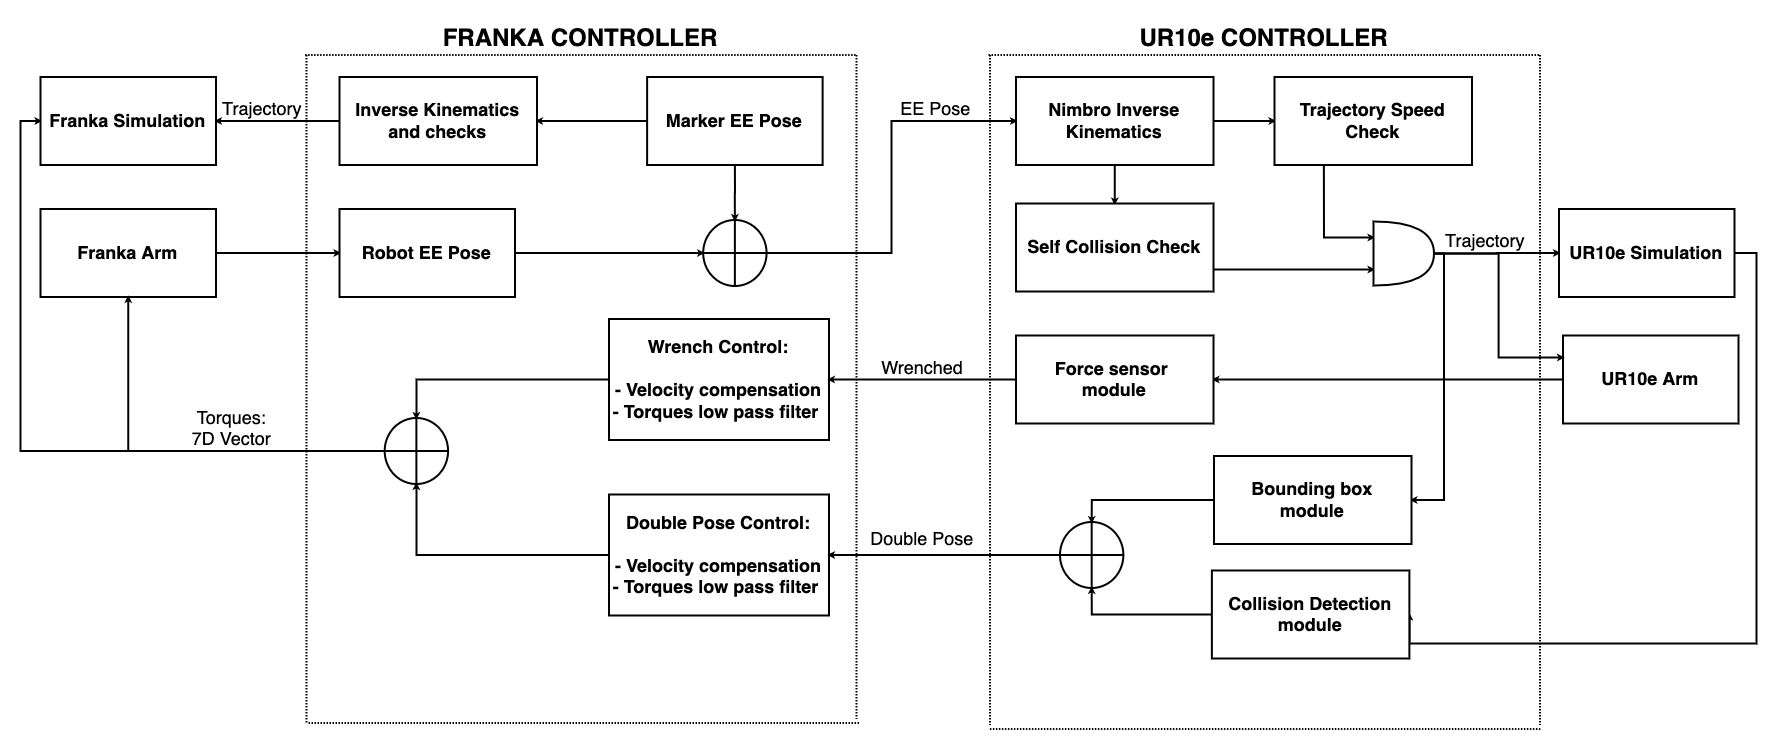
\includegraphics[width=\linewidth]{figures/code-architecture.png}
	\end{center}
	\caption{Architecture diagram.}
	\label{fig:architecture_diagram}
\end{figure}

% --------------------
\section{Inverse Kinematics}
\label{section:ik}

% --------------------
\subsection{Theoretical Aspects}
When performing teleoperation using two robotic arms, it is essential to synchronize the motions between both. This means that any change in position of the master arm's end-effector has to be mimicked by the slave arm. To reach the required end-effector pose on this arm, we use the concept of inverse kinematics.

% "Out project" or "Our project" -> done
% after the two points it is not that fulid the reading

To introduce inverse kinematics, let us first consider the geometry of robotic arms as they are used in our project: Such robots are mounted onto a ground like e.g. a table. Starting from their base, they are combinations of serially connected fixed links and movable (revoluting) joints. At the end of the arm, there is a so-called end-effector which interacts with the environment. This can be a complex grasping device or a simpler tool. The combination of links and joints is referred to as an \textit{(open) kinematic chain}.


% after "inverse kinematics", I think, everything until the end of the paragraph can be shrinked considering that you are expressing only one single concept -> retrieving the endeffecor pose
% third can be improved: "we start .." (in case you want to keep the paragraph)
% sixth line is quite confusing for me "In these coordinate system .." (in case you want to keep the paragraph)

%The pose of the end effector is fully determined by the robot geometry and the joint positions, i.e. angles. The operation to calculate this pose is called \textit{forward kinematics} and consists of several coordinate transforms to sequentially incorporate the joint angles to calculate the poses of the links and finally of the end-effector. The parameters for determining the coordinate transformations (in homogeneous coordinates) are called \textit{Denavit-Hartenberg parameters} and are given in \cite{panda_denavit-hartenberg} for the Franka Emika Panda.

When mimicking the \textit{Panda}'s motions on the \textit{UR10e}, it is not sufficient to transfer the measured joint angles to it. The reason is that first, both robots have a different overall geometry and second, the \textit{UR10e} only has 6 DoF while the \textit{Panda} has 7 DoF. So we have to determine the \textit{UR10e} joint angles from the \textit{Panda}'s end-effector pose. This operation is called \textit{inverse kinematics}.

% third line "Therefore ..." can be connected with the following sentence so you dont repeat two times "the solution"
% "with which" -> "in which": sounds better

Inverse kinematics is a difficult problem to solve compared to forward kinematics. This because in general, there is an infinite number of joint angle combinations that yield a given end-effector pose. Therefore, numerical approaches are used in order to find a possible solution, which is heavily influenced by the initial joint angles the algorithm is provided with.
Instead of implementing an inverse kinematics algorithm on our own, we used the existing implementation described in \cite{schwarz2017nimbro} (\textit{NimbRo IK}).

% why not to devide the topics with subsection? Me and Ilyass did in this way and it seems that can give a brake to the reader and understand the differences between the topics

\subsection{Practical Considerations}
As the mathematical derivation of inverse kinematics was not part of our project, we put more focus on the practical considerations when using inverse kinematics.

% fifth line: "Both arms ..." -> "The arms ..." this will remove the repetition (or maybe you can connect the sentences)
As stated before, the initial position of the robot for which the inverse kinematics is performed is highly important. To get good results in terms of smooth joint trajectories, it is important to always run the algorithm starting from the last known position of the robot (in this case the \textit{UR10e}). The same holds for the initialization of both the \textit{Panda} and the \textit{UR10e}. The robots have to be in an aligned pose, i.e. equivalent despite an offset due to the different position of the robots in space. Unaligned robots would result in a very fast movement of the \textit{UR10e} in the first iteration, possibly causing damage to the robot or environment.

% From "We implmeted (to) MoveIt!" Is not that important and I guess can be removed
% "If a self-collision is detected ..." is past, then also the following verb "send" should be in the past
% 0.5 kHz or 500 Hz: we have this information in three sections and we have to make it consistent (or even remove it considering the repetition of the information)

Furthermore, the inverse kinematics implementation does not prevent self-collisions or arbitrarily high joint speeds by itself, so we added measures for this. If a self-collision is detected in the inverse kinematics' result, the resulting joint angles are not sent to the \textit{UR10e} as a command but the whole program is stopped to prevent damage. For the joint speed limitation, we implemented an upper bound of $1\ \frac{\mathrm{rad}}{\mathrm{s}}$. Given the operating frequency of the \textit{UR10e}, we compute the actual planned speed from the previous joint angles and those computed by the inverse kinematics. If it exceeds the limit, we stop the whole program. This is done because the \textit{Panda} has already been moved in a way that would cause a too fast motion of the \textit{UR10e}, rendering the state unresolvable with respect to aligning the robots again.

% first two sentence can be connected

Another important aspect are singular positions. These describe states in which moving the end-effector in a given new position could be done equivalently by moving one or another joint. This happens e.g. if a robotic arm is straightened to full length. If the \textit{UR10e} gets into such a configuration and the \textit{Panda} is slightly moved, the inverse kinematics does not converge because there are multiple solutions which are too similar with respect to the effort required (i.e. costs). Thus, it is important to avoid such configurations when operating both robotic arms.

% this last line made me cry hahahha

As it was not possible to work with the real robots in the last week of our lab, we used the inverse kinematics for controlling a simulated \textit{Panda} with an interactive marker in \textit{RViz} as well.

% --------------------
\section{Force-Feedback}
\label{section:ff}
% --------------------

Force-feedback is a crucial feature for teleoperated systems, as without knowledge of sensed forces by the slave arm due to collisions with the surroundings, it would be difficult if not impossible to operate in a remote location. In our project we identify two types of forces from two different situations: a simulated collision with either a bounding box or geometric structures, and real forces perceived through a sensor.


\subsection{Collision detection}

Detecting a state of collision is the first necessary step before being able to generate torques corresponding to the experienced forces from the slave arm. In real-world applications, a sensor can extract \textit{wrench forces} perceived from the end-effector joint, expressed by a 6D vector. Besides, force can be simulated. We introduce two types of scenarios were it is possible to simulate collision situations: a \textit{bounding box} defines an imaginary finite topological space where the arm is able to move freely inside but not allowed to exceed its limits, and several \textit{geometric structures} which the slave arm can interact with in a simulation world. The detection of collisions is then defined by the computation of the \textit{closest allowed pose} to the respective box or geometry \textit{surface}.

% ---------------------------
The bounding box is defined by two different thresholds for each coordinate in a 3D space, $min$ and $max$, that indicate the imaginary limits for the robot. For example, if we want to define a cube box that has 1 meter side length, then the thresholds for every single coordinate would be: $ min = -0.5,\ max = 0.5 $.
The surface pose $X_s = [x,y,z]$ is obtained by checking for every coordinate $ k \in \left\{x,y,z\right\} $ if it exceeded its limits or not. In the first case it is assigned the closest limit, otherwise the actual position:

\begin{equation}
k =
\begin{cases}
max, &  k \ge max \\
min, & k \leq min \\
k, & otherwise
\end{cases}
\end{equation}

% ---------------------------

Regarding geometry structures, the closest allowed pose is given by three main information obtained after a collision: the current \textit{pose} of the robot, the \textit{normal} direction and the \textit{depth} of the collision.
\begin{equation}
surface = pose + norm * depth
\end{equation}

% ---------------------------

\subsection{Force generation}

In simulated collisions, the computation of the closest allowed pose enables the generation of torque forces able to drive the arm from a collision state to a non-collision one. Assuming that $X_c$ and $X_s$ are respectively the collision pose and current pose of the master arm represented by two 6D vectors, then the force to use is simply the difference between the two: $ \Delta X = X_s - X_c $. Such force is increased by first multiplying it with a scalar value $\alpha$, and then applying a quadratic function that preserves the sign, in order to increase the force with respect to the distance of the surface.

Finally, we multiply the transposed \textit{Jacobian} matrix with the computed end-effector force obtaining \textit{joint torques} (cf. \cite{rrl}):

\begin{equation}
	F_q = J_{ee}^T  F_{x}
	\label{eq:torqueF}
\end{equation}

If forces are not generated through simulated collisions, but perceived through a force-torque sensor attached to the end-effector of the slave arm, the above formula \eqref{eq:torqueF} can still be used.


\subsection{Control}

Two control loops were implemented to create a force-feedback behavior, depending on whether the force is a simulated one or coming from a force sensor. However, in order to send torques commands to the master arm, these forces need to be converted to a joint space. What follows is a brief explanation of the \textit{Jacobian}, and how this is used for force relation, as well as safety checks introduced in the control loops.

\subsubsection{Jacobian}

Assume a manipulator to be at a specific configuration, denoted as $q$, and whose joints undertook a set of infinitesimally small displacements, represented by the vector $\delta q$. At the end-effector there will be a corresponding set of displacements of its position and orientation $x$, represented by the vector $\delta x$ (cf. \cite{itr}). A general function $f$, representing the forward kinematics model of the manipulator, maps the space defined by the variable $q$ to the space defined by the variable $x$, thereby obtaining a linear system of equations as described in \cite{itr}. If we differentiate the function $f$ with respect to the joints, we get (taken from \cite{itr}):

\begin{equation}
\delta x = \begin{bmatrix}
\frac{\partial f_{1}}{\partial q_{1}} & \ldots & \frac{\partial f_{1}}{\partial q_{n}} \\
\vdots & \vdots & \vdots \\
\frac{\partial f_{m}}{\partial q_{1}} & \ldots & \frac{\partial f_{m}}{\partial q_{n}}
\end{bmatrix} \delta q
\end{equation}

The obtained matrix is the \textit{Jacobian}, which allows us to relate between the velocities of the manipulator in joint and Cartesian space (see \cite{itr}):

\begin{equation}
\label{eqn:jacobian_relation}
\dot{x} = J(q) \dot{q}
\end{equation}

\subsubsection{Force Relation}

The \textit{Jacobian} can also be used to relate between end-effector forces and joint torques. Let us now introduce the physical quantity of \textit{work} which measures the amount of energy transferred when a force is applied over a distance, and \textit{power}, that represents the rate at which work is carried out (cf. \cite{rrl}). If we substitute the equation of \textit{work} into the equation of \textit{power}, and rewrite the obtained relation in terms of the end-effector space as shown in \cite{itr} we get:

\begin{equation}
\label{eqn:ee_eq}
P = F_x^T \dot{x}
\end{equation}

where $F_x$ and $\dot{x}$ are respectively the force vector of the end-effector and its velocity. Through energy equivalence and by carrying out algebraic substitutions we obtain (cf. \cite{rrl}):

\begin{equation}
\label{eqn:step4}
F_q = J_{ee}^T F_x,
\end{equation}

where $J_{ee}(q)$ is exactly the \textit{Jacobian} matrix introduced previously, $F_q$ the forces in joint-space, and $F_x$ the end-effector forces. Therefore, in our control loops, in order to relate between end-effector forces and joint torques, the \textit{Jacobian} is used as described above while considering for \textit{Coriolis} forces. The \textit{Jacobian} gets updated in every loop iteration via the \textit{Franka API}.

\subsection{Velocity Compensation}

To avoid joint velocity limits being reached, a velocity compensation is introduced on the \textit{Panda} arm. At every iteration we compute what future velocities will look like within a given time-step, using current joints' velocity and acceleration. If a future velocity violation is identified, a countering force is computed and added to the original end-effector force to counter the fast movement.

\subsection{Torques Filtering}

If torques were sent directly to the arm, there might be the risk of sudden and sharp forces being commanded. In order to avoid such a scenario, a filtering process is run on the computed joint torques before these are actually applied to the arm. The filter not only checks for limit violations but also acts as a low-pass filter.

% --------------------
\section{Evaluation}
% --------------------
The last week of the lab was planned for fine-tuning the implementation and to carry out a structured evaluation. Nevertheless, this could not be done due to the lockdown caused by the COVID-19 pandemic and the fact that the real \textit{UR10e} robotic arm would have only been available then. The simulated teleoperation completely done in \textit{RViz} does not offer aspects to evaluate with respect to the initially planned project. However, some knowledge about the actual performance of our system was gained before the lockdown allowing some evaluation.

The Panda arm offers real-time communication at a rate of 1 kHz (see \cite{fcid}) and the UR10e arm at 500 Hz (see \cite{urd}). Using the assigned workstation, the communication worked smoothly with a direct connection to the Panda arm. We never experienced any latency while testing the force-feedback using both the virtual bounding box and the standalone force-torque sensor.

The force-feedback itself felt quite realistic. In fact, when the Panda arm is inside the virtual bounding box, it floats freely as one would expect. If it is pushed against a ``wall'', it really feels like touching a soft wall. We only experienced some issues when colliding with the upper plane of the virtual bounding box, as the force-feedback was quite rough. By the end of the last week with the real robot, we could not determine the reason for this. The force-feedback was also tested with the standalone force-torque sensor to mimic the forces that would be transmitted from the \textit{UR10e} arm. In this case, the forces felt even more realistic and there were no random peeks in the force experienced, indicating that the implemented low-pass filter successfully filters erroneous measurements.

Finally, it is worth to note that our implementation is flexible with respect to the used slave robotic arm. For instance, we were first asked to use the \textit{UR5} robotic arm as slave arm. When switching to the \textit{UR10e}, we then only had to exchange the robot description (\textit{URDF} model) to adapt our software.

% --------------------
\section{Conclusions}
% --------------------

The initial aim of developing a teleoperation system with force-feedback capabilities has been successfully met with good results. The system can be used in real-time, with minimal latencies, and realistic force-feedback. Furthermore, a simulated environment was created, so as to allow testing and development without the need of hardware equipment. In the future, a possible improvement could be enhancing the force-feedback behavior when colliding with the upper plane of the virtual bounding box, as this is sometimes too rough. Moreover, an initial synchronization of the two end-effector poses when starting the system should also be implemented to achieve a safer operation.

\bibliography{references.bib}
\end{document}
